\documentclass[1p]{elsarticle_modified}
%\bibliographystyle{elsarticle-num}

%\usepackage[colorlinks]{hyperref}
%\usepackage{abbrmath_seonhwa} %\Abb, \Ascr, \Acal ,\Abf, \Afrak
\usepackage{amsfonts}
\usepackage{amssymb}
\usepackage{amsmath}
\usepackage{amsthm}
\usepackage{scalefnt}
\usepackage{amsbsy}
\usepackage{kotex}
\usepackage{caption}
\usepackage{subfig}
\usepackage{color}
\usepackage{graphicx}
\usepackage{xcolor} %% white, black, red, green, blue, cyan, magenta, yellow
\usepackage{float}
\usepackage{setspace}
\usepackage{hyperref}

\usepackage{tikz}
\usetikzlibrary{arrows}

\usepackage{multirow}
\usepackage{array} % fixed length table
\usepackage{hhline}

%%%%%%%%%%%%%%%%%%%%%
\makeatletter
\renewcommand*\env@matrix[1][\arraystretch]{%
	\edef\arraystretch{#1}%
	\hskip -\arraycolsep
	\let\@ifnextchar\new@ifnextchar
	\array{*\c@MaxMatrixCols c}}
\makeatother %https://tex.stackexchange.com/questions/14071/how-can-i-increase-the-line-spacing-in-a-matrix
%%%%%%%%%%%%%%%

\usepackage[normalem]{ulem}

\newcommand{\msout}[1]{\ifmmode\text{\sout{\ensuremath{#1}}}\else\sout{#1}\fi}
%SOURCE: \msout is \stkout macro in https://tex.stackexchange.com/questions/20609/strikeout-in-math-mode

\newcommand{\cancel}[1]{
	\ifmmode
	{\color{red}\msout{#1}}
	\else
	{\color{red}\sout{#1}}
	\fi
}

\newcommand{\add}[1]{
	{\color{blue}\uwave{#1}}
}

\newcommand{\replace}[2]{
	\ifmmode
	{\color{red}\msout{#1}}{\color{blue}\uwave{#2}}
	\else
	{\color{red}\sout{#1}}{\color{blue}\uwave{#2}}
	\fi
}

\newcommand{\Sol}{\mathcal{S}} %segment
\newcommand{\D}{D} %diagram
\newcommand{\A}{\mathcal{A}} %arc


%%%%%%%%%%%%%%%%%%%%%%%%%%%%%5 test

\def\sl{\operatorname{\textup{SL}}(2,\Cbb)}
\def\psl{\operatorname{\textup{PSL}}(2,\Cbb)}
\def\quan{\mkern 1mu \triangleright \mkern 1mu}

\theoremstyle{definition}
\newtheorem{thm}{Theorem}[section]
\newtheorem{prop}[thm]{Proposition}
\newtheorem{lem}[thm]{Lemma}
\newtheorem{ques}[thm]{Question}
\newtheorem{cor}[thm]{Corollary}
\newtheorem{defn}[thm]{Definition}
\newtheorem{exam}[thm]{Example}
\newtheorem{rmk}[thm]{Remark}
\newtheorem{alg}[thm]{Algorithm}

\newcommand{\I}{\sqrt{-1}}
\begin{document}

%\begin{frontmatter}
%
%\title{Boundary parabolic representations of knots up to 8 crossings}
%
%%% Group authors per affiliation:
%\author{Yunhi Cho} 
%\address{Department of Mathematics, University of Seoul, Seoul, Korea}
%\ead{yhcho@uos.ac.kr}
%
%
%\author{Seonhwa Kim} %\fnref{s_kim}}
%\address{Center for Geometry and Physics, Institute for Basic Science, Pohang, 37673, Korea}
%\ead{ryeona17@ibs.re.kr}
%
%\author{Hyuk Kim}
%\address{Department of Mathematical Sciences, Seoul National University, Seoul 08826, Korea}
%\ead{hyukkim@snu.ac.kr}
%
%\author{Seokbeom Yoon}
%\address{Department of Mathematical Sciences, Seoul National University, Seoul, 08826,  Korea}
%\ead{sbyoon15@snu.ac.kr}
%
%\begin{abstract}
%We find all boundary parabolic representation of knots up to 8 crossings.
%
%\end{abstract}
%\begin{keyword}
%    \MSC[2010] 57M25 
%\end{keyword}
%
%\end{frontmatter}

%\linenumbers
%\tableofcontents
%
\newcommand\colored[1]{\textcolor{white}{\rule[-0.35ex]{0.8em}{1.4ex}}\kern-0.8em\color{red} #1}%
%\newcommand\colored[1]{\textcolor{white}{ #1}\kern-2.17ex	\textcolor{white}{ #1}\kern-1.81ex	\textcolor{white}{ #1}\kern-2.15ex\color{red}#1	}

{\Large $\underline{12a_{0053}~(K12a_{0053})}$}

\setlength{\tabcolsep}{10pt}
\renewcommand{\arraystretch}{1.6}
\vspace{1cm}\begin{tabular}{m{100pt}>{\centering\arraybackslash}m{274pt}}
\multirow{5}{120pt}{
	\centering
	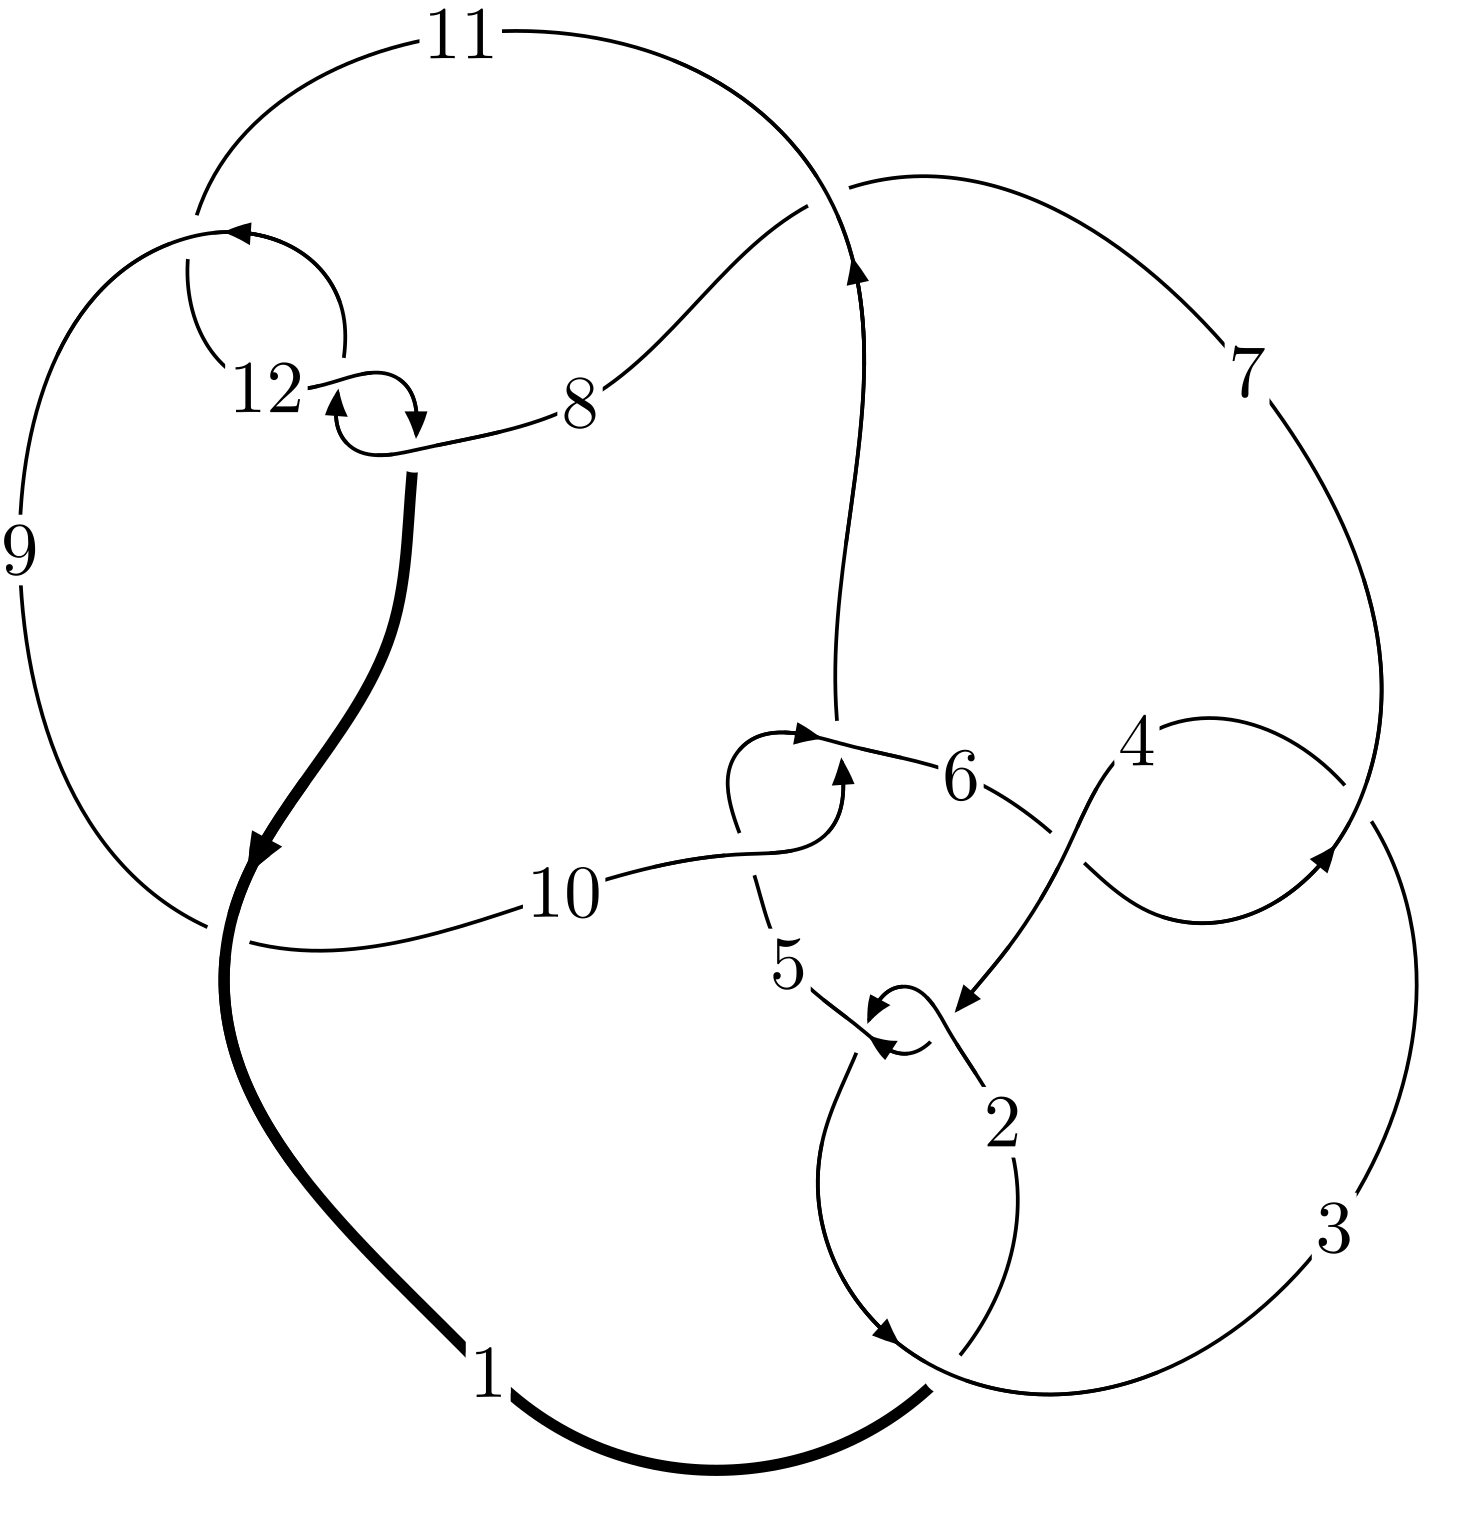
\includegraphics[width=112pt]{../../../GIT/diagram.site/Diagrams/png/854_12a_0053.png}\\
\ \ \ A knot diagram\footnotemark}&
\allowdisplaybreaks
\textbf{Linearized knot diagam} \\
\cline{2-2}
 &
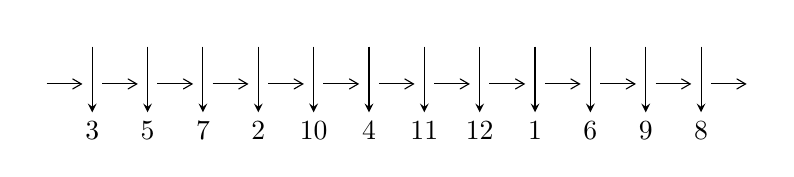
\begin{tikzpicture}[x=20pt, y=17pt]
	% nodes
	\node (C0) at (0, 0) {};
	\node (C1) at (1, 0) {};
	\node (C1U) at (1, +1) {};
	\node (C1D) at (1, -1) {3};

	\node (C2) at (2, 0) {};
	\node (C2U) at (2, +1) {};
	\node (C2D) at (2, -1) {5};

	\node (C3) at (3, 0) {};
	\node (C3U) at (3, +1) {};
	\node (C3D) at (3, -1) {7};

	\node (C4) at (4, 0) {};
	\node (C4U) at (4, +1) {};
	\node (C4D) at (4, -1) {2};

	\node (C5) at (5, 0) {};
	\node (C5U) at (5, +1) {};
	\node (C5D) at (5, -1) {10};

	\node (C6) at (6, 0) {};
	\node (C6U) at (6, +1) {};
	\node (C6D) at (6, -1) {4};

	\node (C7) at (7, 0) {};
	\node (C7U) at (7, +1) {};
	\node (C7D) at (7, -1) {11};

	\node (C8) at (8, 0) {};
	\node (C8U) at (8, +1) {};
	\node (C8D) at (8, -1) {12};

	\node (C9) at (9, 0) {};
	\node (C9U) at (9, +1) {};
	\node (C9D) at (9, -1) {1};

	\node (C10) at (10, 0) {};
	\node (C10U) at (10, +1) {};
	\node (C10D) at (10, -1) {6};

	\node (C11) at (11, 0) {};
	\node (C11U) at (11, +1) {};
	\node (C11D) at (11, -1) {9};

	\node (C12) at (12, 0) {};
	\node (C12U) at (12, +1) {};
	\node (C12D) at (12, -1) {8};
	\node (C13) at (13, 0) {};

	% arrows
	\draw[->,>={angle 60}]
	(C0) edge (C1) (C1) edge (C2) (C2) edge (C3) (C3) edge (C4) (C4) edge (C5) (C5) edge (C6) (C6) edge (C7) (C7) edge (C8) (C8) edge (C9) (C9) edge (C10) (C10) edge (C11) (C11) edge (C12) (C12) edge (C13) ;	\draw[->,>=stealth]
	(C1U) edge (C1D) (C2U) edge (C2D) (C3U) edge (C3D) (C4U) edge (C4D) (C5U) edge (C5D) (C6U) edge (C6D) (C7U) edge (C7D) (C8U) edge (C8D) (C9U) edge (C9D) (C10U) edge (C10D) (C11U) edge (C11D) (C12U) edge (C12D) ;
	\end{tikzpicture} \\
\hhline{~~} \\& 
\textbf{Solving Sequence} \\ \cline{2-2} 
 &
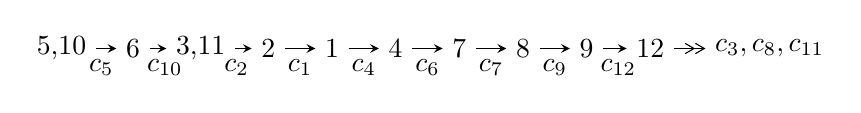
\begin{tikzpicture}[x=23pt, y=7pt]
	% node
	\node (A0) at (-1/8, 0) {5,10};
	\node (A1) at (1, 0) {6};
	\node (A2) at (33/16, 0) {3,11};
	\node (A3) at (25/8, 0) {2};
	\node (A4) at (33/8, 0) {1};
	\node (A5) at (41/8, 0) {4};
	\node (A6) at (49/8, 0) {7};
	\node (A7) at (57/8, 0) {8};
	\node (A8) at (65/8, 0) {9};
	\node (A9) at (73/8, 0) {12};
	\node (C1) at (1/2, -1) {$c_{5}$};
	\node (C2) at (3/2, -1) {$c_{10}$};
	\node (C3) at (21/8, -1) {$c_{2}$};
	\node (C4) at (29/8, -1) {$c_{1}$};
	\node (C5) at (37/8, -1) {$c_{4}$};
	\node (C6) at (45/8, -1) {$c_{6}$};
	\node (C7) at (53/8, -1) {$c_{7}$};
	\node (C8) at (61/8, -1) {$c_{9}$};
	\node (C9) at (69/8, -1) {$c_{12}$};
	\node (A10) at (11, 0) {$c_{3},c_{8},c_{11}$};

	% edge
	\draw[->,>=stealth]	
	(A0) edge (A1) (A1) edge (A2) (A2) edge (A3) (A3) edge (A4) (A4) edge (A5) (A5) edge (A6) (A6) edge (A7) (A7) edge (A8) (A8) edge (A9) ;
	\draw[->>,>={angle 60}]	
	(A9) edge (A10);
\end{tikzpicture} \\ 

\end{tabular} \\

\footnotetext{
The image of knot diagram is generated by the software ``\textbf{Draw programme}" developed by Andrew Bartholomew(\url{http://www.layer8.co.uk/maths/draw/index.htm\#Running-draw}), where we modified some parts for our purpose(\url{https://github.com/CATsTAILs/LinksPainter}).
}\phantom \\ \newline 
\centering \textbf{Ideals for irreducible components\footnotemark of $X_{\text{par}}$} 
 
\begin{align*}
I^u_{1}&=\langle 
-3.63164\times10^{260} u^{101}+2.67815\times10^{260} u^{100}+\cdots+1.75319\times10^{262} b-2.53854\times10^{263},\\
\phantom{I^u_{1}}&\phantom{= \langle  }-1.79420\times10^{261} u^{101}+8.56337\times10^{260} u^{100}+\cdots+7.01276\times10^{262} a-7.92227\times10^{263},\\
\phantom{I^u_{1}}&\phantom{= \langle  }u^{102}-2 u^{101}+\cdots-1024 u-512\rangle \\
I^u_{2}&=\langle 
b+1,\;u^5-4 u^3- u^2+a+4 u+3,\;u^6- u^5-3 u^4+2 u^3+2 u^2+u-1\rangle \\
\\
I^v_{1}&=\langle 
a,\;v^2+b+2 v,\;v^3+3 v^2+2 v+1\rangle \\
I^v_{2}&=\langle 
a,\;-6 v^5+29 v^4-57 v^3-43 v^2+10 b+2 v-1,\;v^6-5 v^5+10 v^4+7 v^3-4 v^2-2 v+1\rangle \\
\end{align*}
\raggedright * 4 irreducible components of $\dim_{\mathbb{C}}=0$, with total 117 representations.\\
\footnotetext{All coefficients of polynomials are rational numbers. But the coefficients are sometimes approximated in decimal forms when there is not enough margin.}
\newpage
\renewcommand{\arraystretch}{1}
\centering \section*{I. $I^u_{1}= \langle -3.63\times10^{260} u^{101}+2.68\times10^{260} u^{100}+\cdots+1.75\times10^{262} b-2.54\times10^{263},\;-1.79\times10^{261} u^{101}+8.56\times10^{260} u^{100}+\cdots+7.01\times10^{262} a-7.92\times10^{263},\;u^{102}-2 u^{101}+\cdots-1024 u-512 \rangle$}
\flushleft \textbf{(i) Arc colorings}\\
\begin{tabular}{m{7pt} m{180pt} m{7pt} m{180pt} }
\flushright $a_{5}=$&$\begin{pmatrix}1\\0\end{pmatrix}$ \\
\flushright $a_{10}=$&$\begin{pmatrix}0\\u\end{pmatrix}$ \\
\flushright $a_{6}=$&$\begin{pmatrix}1\\u^2\end{pmatrix}$ \\
\flushright $a_{3}=$&$\begin{pmatrix}0.0255848 u^{101}-0.0122111 u^{100}+\cdots+83.4661 u+11.2969\\0.0207145 u^{101}-0.0152759 u^{100}+\cdots+31.4829 u+14.4796\end{pmatrix}$ \\
\flushright $a_{11}=$&$\begin{pmatrix}- u\\- u^3+u\end{pmatrix}$ \\
\flushright $a_{2}=$&$\begin{pmatrix}0.0462992 u^{101}-0.0274870 u^{100}+\cdots+114.949 u+25.7765\\0.0207145 u^{101}-0.0152759 u^{100}+\cdots+31.4829 u+14.4796\end{pmatrix}$ \\
\flushright $a_{1}=$&$\begin{pmatrix}-0.0274317 u^{101}+0.0331153 u^{100}+\cdots-44.0458 u-25.7039\\0.0488757 u^{101}-0.0591895 u^{100}+\cdots+95.3012 u+28.8088\end{pmatrix}$ \\
\flushright $a_{4}=$&$\begin{pmatrix}0.0272415 u^{101}-0.00262615 u^{100}+\cdots+74.8617 u+22.1520\\0.0457661 u^{101}-0.0510031 u^{100}+\cdots+104.242 u+36.2491\end{pmatrix}$ \\
\flushright $a_{7}=$&$\begin{pmatrix}0.0214440 u^{101}-0.0260743 u^{100}+\cdots+51.2554 u+3.10487\\-0.0386065 u^{101}+0.0480052 u^{100}+\cdots-67.1046 u-20.2002\end{pmatrix}$ \\
\flushright $a_{8}=$&$\begin{pmatrix}0.0429892 u^{101}-0.0538624 u^{100}+\cdots+87.5705 u+14.2399\\-0.0455989 u^{101}+0.0579958 u^{100}+\cdots-76.7190 u-23.5004\end{pmatrix}$ \\
\flushright $a_{9}=$&$\begin{pmatrix}0.0657508 u^{101}-0.101129 u^{100}+\cdots+110.895 u+1.93899\\-0.0556268 u^{101}+0.0657875 u^{100}+\cdots-118.941 u-39.5496\end{pmatrix}$ \\
\flushright $a_{12}=$&$\begin{pmatrix}-0.0157934 u^{101}+0.0415356 u^{100}+\cdots+36.6963 u+23.0326\\0.00311735 u^{101}+0.00656623 u^{100}+\cdots-7.45847 u+6.07217\end{pmatrix}$\\&\end{tabular}
\flushleft \textbf{(ii) Obstruction class $= -1$}\\~\\
\flushleft \textbf{(iii) Cusp Shapes $= 0.0103007 u^{101}+0.100685 u^{100}+\cdots-40.1004 u+18.3924$}\\~\\
\newpage\renewcommand{\arraystretch}{1}
\flushleft \textbf{(iv) u-Polynomials at the component}\newline \\
\begin{tabular}{m{50pt}|m{274pt}}
Crossings & \hspace{64pt}u-Polynomials at each crossing \\
\hline $$\begin{aligned}c_{1}\end{aligned}$$&$\begin{aligned}
&u^{102}+50 u^{101}+\cdots+200 u+1
\end{aligned}$\\
\hline $$\begin{aligned}c_{2},c_{4}\end{aligned}$$&$\begin{aligned}
&u^{102}-10 u^{101}+\cdots-100 u^2+1
\end{aligned}$\\
\hline $$\begin{aligned}c_{3},c_{6}\end{aligned}$$&$\begin{aligned}
&u^{102}-4 u^{101}+\cdots+384 u-64
\end{aligned}$\\
\hline $$\begin{aligned}c_{5},c_{10}\end{aligned}$$&$\begin{aligned}
&u^{102}-2 u^{101}+\cdots-1024 u-512
\end{aligned}$\\
\hline $$\begin{aligned}c_{7},c_{9}\end{aligned}$$&$\begin{aligned}
&u^{102}+5 u^{101}+\cdots+22859 u+3137
\end{aligned}$\\
\hline $$\begin{aligned}c_{8},c_{11},c_{12}\end{aligned}$$&$\begin{aligned}
&u^{102}-5 u^{101}+\cdots+3 u+1
\end{aligned}$\\
\hline
\end{tabular}\\~\\
\newpage\renewcommand{\arraystretch}{1}
\flushleft \textbf{(v) Riley Polynomials at the component}\newline \\
\begin{tabular}{m{50pt}|m{274pt}}
Crossings & \hspace{64pt}Riley Polynomials at each crossing \\
\hline $$\begin{aligned}c_{1}\end{aligned}$$&$\begin{aligned}
&y^{102}+14 y^{101}+\cdots-37224 y+1
\end{aligned}$\\
\hline $$\begin{aligned}c_{2},c_{4}\end{aligned}$$&$\begin{aligned}
&y^{102}-50 y^{101}+\cdots-200 y+1
\end{aligned}$\\
\hline $$\begin{aligned}c_{3},c_{6}\end{aligned}$$&$\begin{aligned}
&y^{102}+48 y^{101}+\cdots-24576 y+4096
\end{aligned}$\\
\hline $$\begin{aligned}c_{5},c_{10}\end{aligned}$$&$\begin{aligned}
&y^{102}-56 y^{101}+\cdots-10878976 y+262144
\end{aligned}$\\
\hline $$\begin{aligned}c_{7},c_{9}\end{aligned}$$&$\begin{aligned}
&y^{102}-71 y^{101}+\cdots+595599577 y+9840769
\end{aligned}$\\
\hline $$\begin{aligned}c_{8},c_{11},c_{12}\end{aligned}$$&$\begin{aligned}
&y^{102}+85 y^{101}+\cdots+57 y+1
\end{aligned}$\\
\hline
\end{tabular}\\~\\
\newpage\flushleft \textbf{(vi) Complex Volumes and Cusp Shapes}
$$\begin{array}{c|c|c}  
\text{Solutions to }I^u_{1}& \I (\text{vol} + \sqrt{-1}CS) & \text{Cusp shape}\\
 \hline 
\begin{aligned}
u &= \phantom{-}0.469735 + 0.883162 I \\
a &= \phantom{-}0.286453 - 0.882567 I \\
b &= \phantom{-}0.479220 + 0.391058 I\end{aligned}
 & \phantom{-}2.77045 - 2.21678 I & \phantom{-0.000000 } 0 \\ \hline\begin{aligned}
u &= \phantom{-}0.469735 - 0.883162 I \\
a &= \phantom{-}0.286453 + 0.882567 I \\
b &= \phantom{-}0.479220 - 0.391058 I\end{aligned}
 & \phantom{-}2.77045 + 2.21678 I & \phantom{-0.000000 } 0 \\ \hline\begin{aligned}
u &= -0.965899 + 0.256296 I \\
a &= -0.99583 - 1.74154 I \\
b &= -1.049970 + 0.394446 I\end{aligned}
 & -2.68165 + 2.67345 I & \phantom{-0.000000 } 0 \\ \hline\begin{aligned}
u &= -0.965899 - 0.256296 I \\
a &= -0.99583 + 1.74154 I \\
b &= -1.049970 - 0.394446 I\end{aligned}
 & -2.68165 - 2.67345 I & \phantom{-0.000000 } 0 \\ \hline\begin{aligned}
u &= -0.896724 + 0.456096 I \\
a &= -0.092216 + 0.231496 I \\
b &= \phantom{-}0.429580 + 0.543361 I\end{aligned}
 & \phantom{-}0.100178 - 0.283803 I & \phantom{-0.000000 } 0 \\ \hline\begin{aligned}
u &= -0.896724 - 0.456096 I \\
a &= -0.092216 - 0.231496 I \\
b &= \phantom{-}0.429580 - 0.543361 I\end{aligned}
 & \phantom{-}0.100178 + 0.283803 I & \phantom{-0.000000 } 0 \\ \hline\begin{aligned}
u &= \phantom{-}0.859646 + 0.497283 I \\
a &= -0.52080 + 2.39634 I \\
b &= -0.930896 - 0.466209 I\end{aligned}
 & \phantom{-}3.08017 - 4.18267 I & \phantom{-0.000000 } 0 \\ \hline\begin{aligned}
u &= \phantom{-}0.859646 - 0.497283 I \\
a &= -0.52080 - 2.39634 I \\
b &= -0.930896 + 0.466209 I\end{aligned}
 & \phantom{-}3.08017 + 4.18267 I & \phantom{-0.000000 } 0 \\ \hline\begin{aligned}
u &= -0.664667 + 0.756869 I \\
a &= -0.053899 + 1.310560 I \\
b &= \phantom{-}0.606787 - 0.823071 I\end{aligned}
 & \phantom{-}8.69978 + 0.83422 I & \phantom{-0.000000 } 0 \\ \hline\begin{aligned}
u &= -0.664667 - 0.756869 I \\
a &= -0.053899 - 1.310560 I \\
b &= \phantom{-}0.606787 + 0.823071 I\end{aligned}
 & \phantom{-}8.69978 - 0.83422 I & \phantom{-0.000000 } 0\\
 \hline 
 \end{array}$$\newpage$$\begin{array}{c|c|c}  
\text{Solutions to }I^u_{1}& \I (\text{vol} + \sqrt{-1}CS) & \text{Cusp shape}\\
 \hline 
\begin{aligned}
u &= -0.255024 + 0.958228 I \\
a &= \phantom{-}1.22671 + 1.38675 I \\
b &= -1.047270 - 0.391591 I\end{aligned}
 & \phantom{-}0.18214 - 4.88214 I & \phantom{-0.000000 } 0 \\ \hline\begin{aligned}
u &= -0.255024 - 0.958228 I \\
a &= \phantom{-}1.22671 - 1.38675 I \\
b &= -1.047270 + 0.391591 I\end{aligned}
 & \phantom{-}0.18214 + 4.88214 I & \phantom{-0.000000 } 0 \\ \hline\begin{aligned}
u &= \phantom{-}0.852957 + 0.467639 I \\
a &= -0.358332 - 0.587928 I \\
b &= \phantom{-}0.558508 - 0.610769 I\end{aligned}
 & \phantom{-}5.28770 + 3.54945 I & \phantom{-0.000000 } 0 \\ \hline\begin{aligned}
u &= \phantom{-}0.852957 - 0.467639 I \\
a &= -0.358332 + 0.587928 I \\
b &= \phantom{-}0.558508 + 0.610769 I\end{aligned}
 & \phantom{-}5.28770 - 3.54945 I & \phantom{-0.000000 } 0 \\ \hline\begin{aligned}
u &= -0.458068 + 0.947743 I \\
a &= \phantom{-}0.328346 + 1.239270 I \\
b &= \phantom{-}0.341772 - 0.633589 I\end{aligned}
 & -0.30629 - 1.47045 I & \phantom{-0.000000 } 0 \\ \hline\begin{aligned}
u &= -0.458068 - 0.947743 I \\
a &= \phantom{-}0.328346 - 1.239270 I \\
b &= \phantom{-}0.341772 + 0.633589 I\end{aligned}
 & -0.30629 + 1.47045 I & \phantom{-0.000000 } 0 \\ \hline\begin{aligned}
u &= \phantom{-}0.678873 + 0.626121 I \\
a &= \phantom{-}1.18836 - 1.02645 I \\
b &= -0.757090 + 0.486265 I\end{aligned}
 & \phantom{-}3.62452 - 0.25444 I & -12.00000 + 0. I\phantom{ +0.000000I} \\ \hline\begin{aligned}
u &= \phantom{-}0.678873 - 0.626121 I \\
a &= \phantom{-}1.18836 + 1.02645 I \\
b &= -0.757090 - 0.486265 I\end{aligned}
 & \phantom{-}3.62452 + 0.25444 I & -12.00000 + 0. I\phantom{ +0.000000I} \\ \hline\begin{aligned}
u &= \phantom{-}0.119286 + 0.909951 I \\
a &= \phantom{-}1.22475 - 1.50418 I \\
b &= -1.071070 + 0.323375 I\end{aligned}
 & -3.94455 + 1.08858 I & -17.6433 + 0. I\phantom{ +0.000000I} \\ \hline\begin{aligned}
u &= \phantom{-}0.119286 - 0.909951 I \\
a &= \phantom{-}1.22475 + 1.50418 I \\
b &= -1.071070 - 0.323375 I\end{aligned}
 & -3.94455 - 1.08858 I & -17.6433 + 0. I\phantom{ +0.000000I}\\
 \hline 
 \end{array}$$\newpage$$\begin{array}{c|c|c}  
\text{Solutions to }I^u_{1}& \I (\text{vol} + \sqrt{-1}CS) & \text{Cusp shape}\\
 \hline 
\begin{aligned}
u &= \phantom{-}0.054683 + 0.909702 I \\
a &= \phantom{-}1.07662 + 1.64430 I \\
b &= -1.126830 - 0.260614 I\end{aligned}
 & -0.13399 + 2.63215 I & -12.00000 - 4.25973 I \\ \hline\begin{aligned}
u &= \phantom{-}0.054683 - 0.909702 I \\
a &= \phantom{-}1.07662 - 1.64430 I \\
b &= -1.126830 + 0.260614 I\end{aligned}
 & -0.13399 - 2.63215 I & -12.00000 + 4.25973 I \\ \hline\begin{aligned}
u &= -0.552950 + 0.718959 I \\
a &= -0.470014 - 1.024770 I \\
b &= \phantom{-}1.024520 + 0.708766 I\end{aligned}
 & \phantom{-}7.46771 - 4.86452 I & -5.39463 + 0. I\phantom{ +0.000000I} \\ \hline\begin{aligned}
u &= -0.552950 - 0.718959 I \\
a &= -0.470014 + 1.024770 I \\
b &= \phantom{-}1.024520 - 0.708766 I\end{aligned}
 & \phantom{-}7.46771 + 4.86452 I & -5.39463 + 0. I\phantom{ +0.000000I} \\ \hline\begin{aligned}
u &= \phantom{-}1.077250 + 0.202520 I \\
a &= \phantom{-}1.49875 - 0.60317 I \\
b &= \phantom{-}1.007730 + 0.542878 I\end{aligned}
 & \phantom{-}3.95319 - 1.01949 I & \phantom{-0.000000 } 0 \\ \hline\begin{aligned}
u &= \phantom{-}1.077250 - 0.202520 I \\
a &= \phantom{-}1.49875 + 0.60317 I \\
b &= \phantom{-}1.007730 - 0.542878 I\end{aligned}
 & \phantom{-}3.95319 + 1.01949 I & \phantom{-0.000000 } 0 \\ \hline\begin{aligned}
u &= \phantom{-}0.847792 + 0.305277 I \\
a &= -0.306504 - 1.308290 I \\
b &= \phantom{-}0.816745 + 0.899720 I\end{aligned}
 & \phantom{-}5.48740 - 6.77518 I & -12.0000 + 8.1278 I \\ \hline\begin{aligned}
u &= \phantom{-}0.847792 - 0.305277 I \\
a &= -0.306504 + 1.308290 I \\
b &= \phantom{-}0.816745 - 0.899720 I\end{aligned}
 & \phantom{-}5.48740 + 6.77518 I & -12.0000 - 8.1278 I \\ \hline\begin{aligned}
u &= \phantom{-}0.505238 + 0.996875 I \\
a &= \phantom{-}0.276220 - 1.351900 I \\
b &= \phantom{-}0.335981 + 0.733204 I\end{aligned}
 & \phantom{-}4.20848 + 5.36069 I & \phantom{-0.000000 } 0 \\ \hline\begin{aligned}
u &= \phantom{-}0.505238 - 0.996875 I \\
a &= \phantom{-}0.276220 + 1.351900 I \\
b &= \phantom{-}0.335981 - 0.733204 I\end{aligned}
 & \phantom{-}4.20848 - 5.36069 I & \phantom{-0.000000 } 0\\
 \hline 
 \end{array}$$\newpage$$\begin{array}{c|c|c}  
\text{Solutions to }I^u_{1}& \I (\text{vol} + \sqrt{-1}CS) & \text{Cusp shape}\\
 \hline 
\begin{aligned}
u &= \phantom{-}0.879562 + 0.061987 I \\
a &= -1.67185 - 0.65129 I \\
b &= -1.118850 + 0.248432 I\end{aligned}
 & -3.01354 - 0.43650 I & -16.9920 + 5.6265 I \\ \hline\begin{aligned}
u &= \phantom{-}0.879562 - 0.061987 I \\
a &= -1.67185 + 0.65129 I \\
b &= -1.118850 - 0.248432 I\end{aligned}
 & -3.01354 + 0.43650 I & -16.9920 - 5.6265 I \\ \hline\begin{aligned}
u &= \phantom{-}1.010690 + 0.491378 I \\
a &= -0.304624 + 0.260791 I \\
b &= \phantom{-}0.311768 - 0.732223 I\end{aligned}
 & \phantom{-}1.33313 - 3.20923 I & \phantom{-0.000000 } 0 \\ \hline\begin{aligned}
u &= \phantom{-}1.010690 - 0.491378 I \\
a &= -0.304624 - 0.260791 I \\
b &= \phantom{-}0.311768 + 0.732223 I\end{aligned}
 & \phantom{-}1.33313 + 3.20923 I & \phantom{-0.000000 } 0 \\ \hline\begin{aligned}
u &= -0.697298 + 0.512897 I \\
a &= -0.85017 - 1.31278 I \\
b &= -1.203620 - 0.053436 I\end{aligned}
 & \phantom{-}2.04651 + 2.09519 I & -6.28035 - 5.02967 I \\ \hline\begin{aligned}
u &= -0.697298 - 0.512897 I \\
a &= -0.85017 + 1.31278 I \\
b &= -1.203620 + 0.053436 I\end{aligned}
 & \phantom{-}2.04651 - 2.09519 I & -6.28035 + 5.02967 I \\ \hline\begin{aligned}
u &= \phantom{-}0.415660 + 0.730923 I \\
a &= -0.077135 - 1.102180 I \\
b &= \phantom{-}0.691438 + 0.664577 I\end{aligned}
 & \phantom{-}3.13379 - 1.41013 I & -5.75364 + 1.93454 I \\ \hline\begin{aligned}
u &= \phantom{-}0.415660 - 0.730923 I \\
a &= -0.077135 + 1.102180 I \\
b &= \phantom{-}0.691438 - 0.664577 I\end{aligned}
 & \phantom{-}3.13379 + 1.41013 I & -5.75364 - 1.93454 I \\ \hline\begin{aligned}
u &= -0.978284 + 0.623736 I \\
a &= -0.719027 - 0.315629 I \\
b &= \phantom{-}0.422219 + 0.829820 I\end{aligned}
 & \phantom{-}7.68710 + 4.41199 I & \phantom{-0.000000 } 0 \\ \hline\begin{aligned}
u &= -0.978284 - 0.623736 I \\
a &= -0.719027 + 0.315629 I \\
b &= \phantom{-}0.422219 - 0.829820 I\end{aligned}
 & \phantom{-}7.68710 - 4.41199 I & \phantom{-0.000000 } 0\\
 \hline 
 \end{array}$$\newpage$$\begin{array}{c|c|c}  
\text{Solutions to }I^u_{1}& \I (\text{vol} + \sqrt{-1}CS) & \text{Cusp shape}\\
 \hline 
\begin{aligned}
u &= \phantom{-}0.804564 + 0.094462 I \\
a &= -0.412124 + 1.223020 I \\
b &= \phantom{-}0.928475 - 0.856899 I\end{aligned}
 & \phantom{-}5.15559 - 0.37233 I & -13.56324 + 1.75422 I \\ \hline\begin{aligned}
u &= \phantom{-}0.804564 - 0.094462 I \\
a &= -0.412124 - 1.223020 I \\
b &= \phantom{-}0.928475 + 0.856899 I\end{aligned}
 & \phantom{-}5.15559 + 0.37233 I & -13.56324 - 1.75422 I \\ \hline\begin{aligned}
u &= -1.183540 + 0.152520 I \\
a &= \phantom{-}0.584352 + 0.866013 I \\
b &= -0.327386 - 0.735963 I\end{aligned}
 & -1.90155 - 2.90937 I & \phantom{-0.000000 } 0 \\ \hline\begin{aligned}
u &= -1.183540 - 0.152520 I \\
a &= \phantom{-}0.584352 - 0.866013 I \\
b &= -0.327386 + 0.735963 I\end{aligned}
 & -1.90155 + 2.90937 I & \phantom{-0.000000 } 0 \\ \hline\begin{aligned}
u &= \phantom{-}1.167870 + 0.278365 I \\
a &= \phantom{-}0.687171 - 0.928053 I \\
b &= -0.421218 + 0.731632 I\end{aligned}
 & -5.42236 - 1.22087 I & \phantom{-0.000000 } 0 \\ \hline\begin{aligned}
u &= \phantom{-}1.167870 - 0.278365 I \\
a &= \phantom{-}0.687171 + 0.928053 I \\
b &= -0.421218 - 0.731632 I\end{aligned}
 & -5.42236 + 1.22087 I & \phantom{-0.000000 } 0 \\ \hline\begin{aligned}
u &= -1.161710 + 0.380863 I \\
a &= \phantom{-}0.754334 + 0.984612 I \\
b &= -0.493125 - 0.737361 I\end{aligned}
 & -1.13135 + 5.34314 I & \phantom{-0.000000 } 0 \\ \hline\begin{aligned}
u &= -1.161710 - 0.380863 I \\
a &= \phantom{-}0.754334 - 0.984612 I \\
b &= -0.493125 + 0.737361 I\end{aligned}
 & -1.13135 - 5.34314 I & \phantom{-0.000000 } 0 \\ \hline\begin{aligned}
u &= -0.760304 + 0.132527 I \\
a &= -0.345603 + 1.251750 I \\
b &= \phantom{-}0.865317 - 0.863222 I\end{aligned}
 & \phantom{-}1.28913 + 3.15635 I & -18.6926 - 4.9567 I \\ \hline\begin{aligned}
u &= -0.760304 - 0.132527 I \\
a &= -0.345603 - 1.251750 I \\
b &= \phantom{-}0.865317 + 0.863222 I\end{aligned}
 & \phantom{-}1.28913 - 3.15635 I & -18.6926 + 4.9567 I\\
 \hline 
 \end{array}$$\newpage$$\begin{array}{c|c|c}  
\text{Solutions to }I^u_{1}& \I (\text{vol} + \sqrt{-1}CS) & \text{Cusp shape}\\
 \hline 
\begin{aligned}
u &= -1.118500 + 0.552200 I \\
a &= \phantom{-}0.95395 + 1.54284 I \\
b &= \phantom{-}1.114870 - 0.615352 I\end{aligned}
 & \phantom{-}5.60729 + 9.79157 I & \phantom{-0.000000 } 0 \\ \hline\begin{aligned}
u &= -1.118500 - 0.552200 I \\
a &= \phantom{-}0.95395 - 1.54284 I \\
b &= \phantom{-}1.114870 + 0.615352 I\end{aligned}
 & \phantom{-}5.60729 - 9.79157 I & \phantom{-0.000000 } 0 \\ \hline\begin{aligned}
u &= -1.226270 + 0.279300 I \\
a &= \phantom{-}1.044130 + 0.778399 I \\
b &= \phantom{-}1.067550 - 0.516419 I\end{aligned}
 & -1.78322 + 4.05653 I & \phantom{-0.000000 } 0 \\ \hline\begin{aligned}
u &= -1.226270 - 0.279300 I \\
a &= \phantom{-}1.044130 - 0.778399 I \\
b &= \phantom{-}1.067550 + 0.516419 I\end{aligned}
 & -1.78322 - 4.05653 I & \phantom{-0.000000 } 0 \\ \hline\begin{aligned}
u &= \phantom{-}0.341376 + 0.658757 I \\
a &= \phantom{-}0.850121 - 0.679018 I \\
b &= \phantom{-}0.134755 + 0.186887 I\end{aligned}
 & \phantom{-}2.73869 - 2.12194 I & -5.45556 + 2.97058 I \\ \hline\begin{aligned}
u &= \phantom{-}0.341376 - 0.658757 I \\
a &= \phantom{-}0.850121 + 0.679018 I \\
b &= \phantom{-}0.134755 - 0.186887 I\end{aligned}
 & \phantom{-}2.73869 + 2.12194 I & -5.45556 - 2.97058 I \\ \hline\begin{aligned}
u &= \phantom{-}0.237869 + 1.242390 I \\
a &= -0.439691 + 0.766188 I \\
b &= \phantom{-}1.059290 - 0.500801 I\end{aligned}
 & \phantom{-}0.93403 + 1.83086 I & \phantom{-0.000000 } 0 \\ \hline\begin{aligned}
u &= \phantom{-}0.237869 - 1.242390 I \\
a &= -0.439691 - 0.766188 I \\
b &= \phantom{-}1.059290 + 0.500801 I\end{aligned}
 & \phantom{-}0.93403 - 1.83086 I & \phantom{-0.000000 } 0 \\ \hline\begin{aligned}
u &= \phantom{-}0.131680 + 0.704994 I \\
a &= -0.328865 + 0.986806 I \\
b &= \phantom{-}0.921623 - 0.644162 I\end{aligned}
 & \phantom{-}2.47180 + 3.64125 I & -5.93260 - 6.08823 I \\ \hline\begin{aligned}
u &= \phantom{-}0.131680 - 0.704994 I \\
a &= -0.328865 - 0.986806 I \\
b &= \phantom{-}0.921623 + 0.644162 I\end{aligned}
 & \phantom{-}2.47180 - 3.64125 I & -5.93260 + 6.08823 I\\
 \hline 
 \end{array}$$\newpage$$\begin{array}{c|c|c}  
\text{Solutions to }I^u_{1}& \I (\text{vol} + \sqrt{-1}CS) & \text{Cusp shape}\\
 \hline 
\begin{aligned}
u &= -0.364857 + 1.236950 I \\
a &= -0.495662 - 0.796350 I \\
b &= \phantom{-}1.095170 + 0.535588 I\end{aligned}
 & -2.46443 - 6.07420 I & \phantom{-0.000000 } 0 \\ \hline\begin{aligned}
u &= -0.364857 - 1.236950 I \\
a &= -0.495662 + 0.796350 I \\
b &= \phantom{-}1.095170 - 0.535588 I\end{aligned}
 & -2.46443 + 6.07420 I & \phantom{-0.000000 } 0 \\ \hline\begin{aligned}
u &= \phantom{-}1.258950 + 0.297340 I \\
a &= -0.401660 - 0.297563 I \\
b &= -1.314010 + 0.281641 I\end{aligned}
 & -4.86882 + 0.96261 I & \phantom{-0.000000 } 0 \\ \hline\begin{aligned}
u &= \phantom{-}1.258950 - 0.297340 I \\
a &= -0.401660 + 0.297563 I \\
b &= -1.314010 - 0.281641 I\end{aligned}
 & -4.86882 - 0.96261 I & \phantom{-0.000000 } 0 \\ \hline\begin{aligned}
u &= \phantom{-}0.458497 + 1.227020 I \\
a &= -0.532964 + 0.821965 I \\
b &= \phantom{-}1.118460 - 0.562936 I\end{aligned}
 & \phantom{-}1.92668 + 10.29270 I & \phantom{-0.000000 } 0 \\ \hline\begin{aligned}
u &= \phantom{-}0.458497 - 1.227020 I \\
a &= -0.532964 - 0.821965 I \\
b &= \phantom{-}1.118460 + 0.562936 I\end{aligned}
 & \phantom{-}1.92668 - 10.29270 I & \phantom{-0.000000 } 0 \\ \hline\begin{aligned}
u &= \phantom{-}1.187880 + 0.553524 I \\
a &= -0.355130 + 0.685776 I \\
b &= \phantom{-}0.239674 - 0.902710 I\end{aligned}
 & \phantom{-}0.19904 - 3.04869 I & \phantom{-0.000000 } 0 \\ \hline\begin{aligned}
u &= \phantom{-}1.187880 - 0.553524 I \\
a &= -0.355130 - 0.685776 I \\
b &= \phantom{-}0.239674 + 0.902710 I\end{aligned}
 & \phantom{-}0.19904 + 3.04869 I & \phantom{-0.000000 } 0 \\ \hline\begin{aligned}
u &= -1.251460 + 0.405072 I \\
a &= -0.311122 + 0.114315 I \\
b &= -1.340840 - 0.245232 I\end{aligned}
 & -8.19580 + 3.31639 I & \phantom{-0.000000 } 0 \\ \hline\begin{aligned}
u &= -1.251460 - 0.405072 I \\
a &= -0.311122 - 0.114315 I \\
b &= -1.340840 + 0.245232 I\end{aligned}
 & -8.19580 - 3.31639 I & \phantom{-0.000000 } 0\\
 \hline 
 \end{array}$$\newpage$$\begin{array}{c|c|c}  
\text{Solutions to }I^u_{1}& \I (\text{vol} + \sqrt{-1}CS) & \text{Cusp shape}\\
 \hline 
\begin{aligned}
u &= -1.250310 + 0.409568 I \\
a &= -0.27505 - 1.58198 I \\
b &= -1.122860 + 0.534778 I\end{aligned}
 & -4.28336 + 1.91291 I & \phantom{-0.000000 } 0 \\ \hline\begin{aligned}
u &= -1.250310 - 0.409568 I \\
a &= -0.27505 + 1.58198 I \\
b &= -1.122860 - 0.534778 I\end{aligned}
 & -4.28336 - 1.91291 I & \phantom{-0.000000 } 0 \\ \hline\begin{aligned}
u &= \phantom{-}1.245540 + 0.444122 I \\
a &= \phantom{-}0.86118 - 1.13024 I \\
b &= \phantom{-}1.119470 + 0.554114 I\end{aligned}
 & -1.00865 - 8.08532 I & \phantom{-0.000000 } 0 \\ \hline\begin{aligned}
u &= \phantom{-}1.245540 - 0.444122 I \\
a &= \phantom{-}0.86118 + 1.13024 I \\
b &= \phantom{-}1.119470 - 0.554114 I\end{aligned}
 & -1.00865 + 8.08532 I & \phantom{-0.000000 } 0 \\ \hline\begin{aligned}
u &= \phantom{-}1.238600 + 0.485737 I \\
a &= -0.238880 + 0.015588 I \\
b &= -1.358710 + 0.216589 I\end{aligned}
 & -3.76353 - 7.55514 I & \phantom{-0.000000 } 0 \\ \hline\begin{aligned}
u &= \phantom{-}1.238600 - 0.485737 I \\
a &= -0.238880 - 0.015588 I \\
b &= -1.358710 - 0.216589 I\end{aligned}
 & -3.76353 + 7.55514 I & \phantom{-0.000000 } 0 \\ \hline\begin{aligned}
u &= \phantom{-}1.248460 + 0.507912 I \\
a &= -0.17120 + 1.69208 I \\
b &= -1.098050 - 0.574579 I\end{aligned}
 & -7.44285 - 6.21744 I & \phantom{-0.000000 } 0 \\ \hline\begin{aligned}
u &= \phantom{-}1.248460 - 0.507912 I \\
a &= -0.17120 - 1.69208 I \\
b &= -1.098050 + 0.574579 I\end{aligned}
 & -7.44285 + 6.21744 I & \phantom{-0.000000 } 0 \\ \hline\begin{aligned}
u &= -1.199110 + 0.632919 I \\
a &= -0.476470 - 0.759573 I \\
b &= \phantom{-}0.281258 + 0.951290 I\end{aligned}
 & -2.72286 + 7.32646 I & \phantom{-0.000000 } 0 \\ \hline\begin{aligned}
u &= -1.199110 - 0.632919 I \\
a &= -0.476470 + 0.759573 I \\
b &= \phantom{-}0.281258 - 0.951290 I\end{aligned}
 & -2.72286 - 7.32646 I & \phantom{-0.000000 } 0\\
 \hline 
 \end{array}$$\newpage$$\begin{array}{c|c|c}  
\text{Solutions to }I^u_{1}& \I (\text{vol} + \sqrt{-1}CS) & \text{Cusp shape}\\
 \hline 
\begin{aligned}
u &= -1.236410 + 0.575925 I \\
a &= -0.10670 - 1.76523 I \\
b &= -1.076880 + 0.600242 I\end{aligned}
 & -2.88830 + 10.46490 I & \phantom{-0.000000 } 0 \\ \hline\begin{aligned}
u &= -1.236410 - 0.575925 I \\
a &= -0.10670 + 1.76523 I \\
b &= -1.076880 - 0.600242 I\end{aligned}
 & -2.88830 - 10.46490 I & \phantom{-0.000000 } 0 \\ \hline\begin{aligned}
u &= \phantom{-}1.192890 + 0.683328 I \\
a &= -0.556877 + 0.795127 I \\
b &= \phantom{-}0.311441 - 0.974383 I\end{aligned}
 & \phantom{-}1.98421 - 11.53410 I & \phantom{-0.000000 } 0 \\ \hline\begin{aligned}
u &= \phantom{-}1.192890 - 0.683328 I \\
a &= -0.556877 - 0.795127 I \\
b &= \phantom{-}0.311441 + 0.974383 I\end{aligned}
 & \phantom{-}1.98421 + 11.53410 I & \phantom{-0.000000 } 0 \\ \hline\begin{aligned}
u &= \phantom{-}1.34180 + 0.63995 I \\
a &= \phantom{-}0.457492 - 1.332140 I \\
b &= \phantom{-}1.196990 + 0.583051 I\end{aligned}
 & -2.67024 - 8.45023 I & \phantom{-0.000000 } 0 \\ \hline\begin{aligned}
u &= \phantom{-}1.34180 - 0.63995 I \\
a &= \phantom{-}0.457492 + 1.332140 I \\
b &= \phantom{-}1.196990 - 0.583051 I\end{aligned}
 & -2.67024 + 8.45023 I & \phantom{-0.000000 } 0 \\ \hline\begin{aligned}
u &= \phantom{-}1.28912 + 0.75340 I \\
a &= \phantom{-}0.36121 - 1.54178 I \\
b &= \phantom{-}1.209450 + 0.627942 I\end{aligned}
 & -0.7652 - 17.3335 I & \phantom{-0.000000 } 0 \\ \hline\begin{aligned}
u &= \phantom{-}1.28912 - 0.75340 I \\
a &= \phantom{-}0.36121 + 1.54178 I \\
b &= \phantom{-}1.209450 - 0.627942 I\end{aligned}
 & -0.7652 + 17.3335 I & \phantom{-0.000000 } 0 \\ \hline\begin{aligned}
u &= -1.31875 + 0.71144 I \\
a &= \phantom{-}0.38934 + 1.45200 I \\
b &= \phantom{-}1.207890 - 0.609037 I\end{aligned}
 & -5.54444 + 12.98070 I & \phantom{-0.000000 } 0 \\ \hline\begin{aligned}
u &= -1.31875 - 0.71144 I \\
a &= \phantom{-}0.38934 - 1.45200 I \\
b &= \phantom{-}1.207890 + 0.609037 I\end{aligned}
 & -5.54444 - 12.98070 I & \phantom{-0.000000 } 0\\
 \hline 
 \end{array}$$\newpage$$\begin{array}{c|c|c}  
\text{Solutions to }I^u_{1}& \I (\text{vol} + \sqrt{-1}CS) & \text{Cusp shape}\\
 \hline 
\begin{aligned}
u &= -0.497844\phantom{ +0.000000I} \\
a &= \phantom{-}0.865204\phantom{ +0.000000I} \\
b &= -0.0717077\phantom{ +0.000000I}\end{aligned}
 & -0.675799\phantom{ +0.000000I} & -14.6910\phantom{ +0.000000I} \\ \hline\begin{aligned}
u &= -0.326069 + 0.266750 I \\
a &= \phantom{-}1.77180 + 0.55149 I \\
b &= -0.719427 - 0.150406 I\end{aligned}
 & -0.978110 - 0.104240 I & -10.05546 - 1.12981 I \\ \hline\begin{aligned}
u &= -0.326069 - 0.266750 I \\
a &= \phantom{-}1.77180 - 0.55149 I \\
b &= -0.719427 + 0.150406 I\end{aligned}
 & -0.978110 + 0.104240 I & -10.05546 + 1.12981 I \\ \hline\begin{aligned}
u &= -0.400500 + 0.102762 I \\
a &= -7.18535 - 4.89337 I \\
b &= -0.879416 + 0.112735 I\end{aligned}
 & \phantom{-}1.77306 - 2.64662 I & -33.5126 - 4.0993 I \\ \hline\begin{aligned}
u &= -0.400500 - 0.102762 I \\
a &= -7.18535 + 4.89337 I \\
b &= -0.879416 - 0.112735 I\end{aligned}
 & \phantom{-}1.77306 + 2.64662 I & -33.5126 + 4.0993 I \\ \hline\begin{aligned}
u &= -1.59121 + 0.07207 I \\
a &= \phantom{-}0.446162 - 0.200488 I \\
b &= \phantom{-}1.058940 + 0.304432 I\end{aligned}
 & -5.92991 - 5.44719 I & \phantom{-0.000000 } 0 \\ \hline\begin{aligned}
u &= -1.59121 - 0.07207 I \\
a &= \phantom{-}0.446162 + 0.200488 I \\
b &= \phantom{-}1.058940 - 0.304432 I\end{aligned}
 & -5.92991 + 5.44719 I & \phantom{-0.000000 } 0 \\ \hline\begin{aligned}
u &= -1.58344 + 0.30802 I \\
a &= \phantom{-}0.395590 - 0.007776 I \\
b &= \phantom{-}0.988167 + 0.243027 I\end{aligned}
 & -5.46115 + 3.91765 I & \phantom{-0.000000 } 0 \\ \hline\begin{aligned}
u &= -1.58344 - 0.30802 I \\
a &= \phantom{-}0.395590 + 0.007776 I \\
b &= \phantom{-}0.988167 - 0.243027 I\end{aligned}
 & -5.46115 - 3.91765 I & \phantom{-0.000000 } 0 \\ \hline\begin{aligned}
u &= \phantom{-}1.60314 + 0.19201 I \\
a &= \phantom{-}0.413865 + 0.095304 I \\
b &= \phantom{-}1.025450 - 0.268432 I\end{aligned}
 & -9.63402 + 0.74509 I & \phantom{-0.000000 } 0\\
 \hline 
 \end{array}$$\newpage$$\begin{array}{c|c|c}  
\text{Solutions to }I^u_{1}& \I (\text{vol} + \sqrt{-1}CS) & \text{Cusp shape}\\
 \hline 
\begin{aligned}
u &= \phantom{-}1.60314 - 0.19201 I \\
a &= \phantom{-}0.413865 - 0.095304 I \\
b &= \phantom{-}1.025450 + 0.268432 I\end{aligned}
 & -9.63402 - 0.74509 I & \phantom{-0.000000 } 0 \\ \hline\begin{aligned}
u &= \phantom{-}0.341325\phantom{ +0.000000I} \\
a &= -10.9115\phantom{ +0.000000I} \\
b &= -0.954265\phantom{ +0.000000I}\end{aligned}
 & -2.53188\phantom{ +0.000000I} & -77.9360\phantom{ +0.000000I}\\
 \hline 
 \end{array}$$\newpage\newpage\renewcommand{\arraystretch}{1}
\centering \section*{II. $I^u_{2}= \langle b+1,\;u^5-4 u^3- u^2+a+4 u+3,\;u^6- u^5-3 u^4+2 u^3+2 u^2+u-1 \rangle$}
\flushleft \textbf{(i) Arc colorings}\\
\begin{tabular}{m{7pt} m{180pt} m{7pt} m{180pt} }
\flushright $a_{5}=$&$\begin{pmatrix}1\\0\end{pmatrix}$ \\
\flushright $a_{10}=$&$\begin{pmatrix}0\\u\end{pmatrix}$ \\
\flushright $a_{6}=$&$\begin{pmatrix}1\\u^2\end{pmatrix}$ \\
\flushright $a_{3}=$&$\begin{pmatrix}- u^5+4 u^3+u^2-4 u-3\\-1\end{pmatrix}$ \\
\flushright $a_{11}=$&$\begin{pmatrix}- u\\- u^3+u\end{pmatrix}$ \\
\flushright $a_{2}=$&$\begin{pmatrix}- u^5+4 u^3+u^2-4 u-4\\-1\end{pmatrix}$ \\
\flushright $a_{1}=$&$\begin{pmatrix}-1\\0\end{pmatrix}$ \\
\flushright $a_{4}=$&$\begin{pmatrix}- u^5+4 u^3+u^2-4 u-3\\-1\end{pmatrix}$ \\
\flushright $a_{7}=$&$\begin{pmatrix}1\\u^2\end{pmatrix}$ \\
\flushright $a_{8}=$&$\begin{pmatrix}- u^2+1\\- u^4+2 u^2\end{pmatrix}$ \\
\flushright $a_{9}=$&$\begin{pmatrix}u\\u\end{pmatrix}$ \\
\flushright $a_{12}=$&$\begin{pmatrix}u^5-2 u^3- u\\u^5-3 u^3+u\end{pmatrix}$\\&\end{tabular}
\flushleft \textbf{(ii) Obstruction class $= 1$}\\~\\
\flushleft \textbf{(iii) Cusp Shapes $= 7 u^5-3 u^4-19 u^3+5 u^2+8 u-6$}\\~\\
\newpage\renewcommand{\arraystretch}{1}
\flushleft \textbf{(iv) u-Polynomials at the component}\newline \\
\begin{tabular}{m{50pt}|m{274pt}}
Crossings & \hspace{64pt}u-Polynomials at each crossing \\
\hline $$\begin{aligned}c_{1},c_{2}\end{aligned}$$&$\begin{aligned}
&(u-1)^6
\end{aligned}$\\
\hline $$\begin{aligned}c_{3},c_{6}\end{aligned}$$&$\begin{aligned}
&u^6
\end{aligned}$\\
\hline $$\begin{aligned}c_{4}\end{aligned}$$&$\begin{aligned}
&(u+1)^6
\end{aligned}$\\
\hline $$\begin{aligned}c_{5},c_{7},c_{9}\end{aligned}$$&$\begin{aligned}
&u^6- u^5-3 u^4+2 u^3+2 u^2+u-1
\end{aligned}$\\
\hline $$\begin{aligned}c_{8}\end{aligned}$$&$\begin{aligned}
&u^6+u^5+3 u^4+2 u^3+2 u^2+u-1
\end{aligned}$\\
\hline $$\begin{aligned}c_{10}\end{aligned}$$&$\begin{aligned}
&u^6+u^5-3 u^4-2 u^3+2 u^2- u-1
\end{aligned}$\\
\hline $$\begin{aligned}c_{11},c_{12}\end{aligned}$$&$\begin{aligned}
&u^6- u^5+3 u^4-2 u^3+2 u^2- u-1
\end{aligned}$\\
\hline
\end{tabular}\\~\\
\newpage\renewcommand{\arraystretch}{1}
\flushleft \textbf{(v) Riley Polynomials at the component}\newline \\
\begin{tabular}{m{50pt}|m{274pt}}
Crossings & \hspace{64pt}Riley Polynomials at each crossing \\
\hline $$\begin{aligned}c_{1},c_{2},c_{4}\end{aligned}$$&$\begin{aligned}
&(y-1)^6
\end{aligned}$\\
\hline $$\begin{aligned}c_{3},c_{6}\end{aligned}$$&$\begin{aligned}
&y^6
\end{aligned}$\\
\hline $$\begin{aligned}c_{5},c_{7},c_{9}\\c_{10}\end{aligned}$$&$\begin{aligned}
&y^6-7 y^5+17 y^4-16 y^3+6 y^2-5 y+1
\end{aligned}$\\
\hline $$\begin{aligned}c_{8},c_{11},c_{12}\end{aligned}$$&$\begin{aligned}
&y^6+5 y^5+9 y^4+4 y^3-6 y^2-5 y+1
\end{aligned}$\\
\hline
\end{tabular}\\~\\
\newpage\flushleft \textbf{(vi) Complex Volumes and Cusp Shapes}
$$\begin{array}{c|c|c}  
\text{Solutions to }I^u_{2}& \I (\text{vol} + \sqrt{-1}CS) & \text{Cusp shape}\\
 \hline 
\begin{aligned}
u &= -0.493180 + 0.575288 I \\
a &= \phantom{-}0.26610 - 1.72116 I \\
b &= -1.00000\phantom{ +0.000000I}\end{aligned}
 & \phantom{-}1.31531 + 1.97241 I & -15.7816 - 4.5012 I \\ \hline\begin{aligned}
u &= -0.493180 - 0.575288 I \\
a &= \phantom{-}0.26610 + 1.72116 I \\
b &= -1.00000\phantom{ +0.000000I}\end{aligned}
 & \phantom{-}1.31531 - 1.97241 I & -15.7816 + 4.5012 I \\ \hline\begin{aligned}
u &= \phantom{-}0.483672\phantom{ +0.000000I} \\
a &= -4.27462\phantom{ +0.000000I} \\
b &= -1.00000\phantom{ +0.000000I}\end{aligned}
 & -2.38379\phantom{ +0.000000I} & -3.08970\phantom{ +0.000000I} \\ \hline\begin{aligned}
u &= \phantom{-}1.52087 + 0.16310 I \\
a &= -0.417699 + 0.090629 I \\
b &= -1.00000\phantom{ +0.000000I}\end{aligned}
 & -5.34051 - 4.59213 I & -11.43321 + 5.39767 I \\ \hline\begin{aligned}
u &= \phantom{-}1.52087 - 0.16310 I \\
a &= -0.417699 - 0.090629 I \\
b &= -1.00000\phantom{ +0.000000I}\end{aligned}
 & -5.34051 + 4.59213 I & -11.43321 - 5.39767 I \\ \hline\begin{aligned}
u &= -1.53904\phantom{ +0.000000I} \\
a &= -0.422181\phantom{ +0.000000I} \\
b &= -1.00000\phantom{ +0.000000I}\end{aligned}
 & -9.30502\phantom{ +0.000000I} & -14.4810\phantom{ +0.000000I}\\
 \hline 
 \end{array}$$\newpage\newpage\renewcommand{\arraystretch}{1}
\centering \section*{III. $I^v_{1}= \langle a,\;v^2+b+2 v,\;v^3+3 v^2+2 v+1 \rangle$}
\flushleft \textbf{(i) Arc colorings}\\
\begin{tabular}{m{7pt} m{180pt} m{7pt} m{180pt} }
\flushright $a_{5}=$&$\begin{pmatrix}1\\0\end{pmatrix}$ \\
\flushright $a_{10}=$&$\begin{pmatrix}v\\0\end{pmatrix}$ \\
\flushright $a_{6}=$&$\begin{pmatrix}1\\0\end{pmatrix}$ \\
\flushright $a_{3}=$&$\begin{pmatrix}0\\- v^2-2 v\end{pmatrix}$ \\
\flushright $a_{11}=$&$\begin{pmatrix}v\\0\end{pmatrix}$ \\
\flushright $a_{2}=$&$\begin{pmatrix}- v^2-2 v\\- v^2-2 v\end{pmatrix}$ \\
\flushright $a_{1}=$&$\begin{pmatrix}- v^2-2 v\\v+2\end{pmatrix}$ \\
\flushright $a_{4}=$&$\begin{pmatrix}v^2+3 v+2\\v^2+3 v+1\end{pmatrix}$ \\
\flushright $a_{7}=$&$\begin{pmatrix}v^2+2 v\\- v-2\end{pmatrix}$ \\
\flushright $a_{8}=$&$\begin{pmatrix}-1\\- v-2\end{pmatrix}$ \\
\flushright $a_{9}=$&$\begin{pmatrix}- v^2-2 v-1\\- v^2-2 v+1\end{pmatrix}$ \\
\flushright $a_{12}=$&$\begin{pmatrix}v+1\\2 v^2+6 v+3\end{pmatrix}$\\&\end{tabular}
\flushleft \textbf{(ii) Obstruction class $= 1$}\\~\\
\flushleft \textbf{(iii) Cusp Shapes $= -5 v^2-11 v-13$}\\~\\
\newpage\renewcommand{\arraystretch}{1}
\flushleft \textbf{(iv) u-Polynomials at the component}\newline \\
\begin{tabular}{m{50pt}|m{274pt}}
Crossings & \hspace{64pt}u-Polynomials at each crossing \\
\hline $$\begin{aligned}c_{1},c_{3},c_{8}\end{aligned}$$&$\begin{aligned}
&u^3- u^2+2 u-1
\end{aligned}$\\
\hline $$\begin{aligned}c_{2},c_{7},c_{9}\end{aligned}$$&$\begin{aligned}
&u^3+u^2-1
\end{aligned}$\\
\hline $$\begin{aligned}c_{4}\end{aligned}$$&$\begin{aligned}
&u^3- u^2+1
\end{aligned}$\\
\hline $$\begin{aligned}c_{5},c_{10}\end{aligned}$$&$\begin{aligned}
&u^3
\end{aligned}$\\
\hline $$\begin{aligned}c_{6},c_{11},c_{12}\end{aligned}$$&$\begin{aligned}
&u^3+u^2+2 u+1
\end{aligned}$\\
\hline
\end{tabular}\\~\\
\newpage\renewcommand{\arraystretch}{1}
\flushleft \textbf{(v) Riley Polynomials at the component}\newline \\
\begin{tabular}{m{50pt}|m{274pt}}
Crossings & \hspace{64pt}Riley Polynomials at each crossing \\
\hline $$\begin{aligned}c_{1},c_{3},c_{6}\\c_{8},c_{11},c_{12}\end{aligned}$$&$\begin{aligned}
&y^3+3 y^2+2 y-1
\end{aligned}$\\
\hline $$\begin{aligned}c_{2},c_{4},c_{7}\\c_{9}\end{aligned}$$&$\begin{aligned}
&y^3- y^2+2 y-1
\end{aligned}$\\
\hline $$\begin{aligned}c_{5},c_{10}\end{aligned}$$&$\begin{aligned}
&y^3
\end{aligned}$\\
\hline
\end{tabular}\\~\\
\newpage\flushleft \textbf{(vi) Complex Volumes and Cusp Shapes}
$$\begin{array}{c|c|c}  
\text{Solutions to }I^v_{1}& \I (\text{vol} + \sqrt{-1}CS) & \text{Cusp shape}\\
 \hline 
\begin{aligned}
v &= -0.337641 + 0.562280 I \\
a &= \phantom{-0.000000 } 0 \\
b &= \phantom{-}0.877439 - 0.744862 I\end{aligned}
 & \phantom{-}6.04826 + 5.65624 I & -8.27516 - 4.28659 I \\ \hline\begin{aligned}
v &= -0.337641 - 0.562280 I \\
a &= \phantom{-0.000000 } 0 \\
b &= \phantom{-}0.877439 + 0.744862 I\end{aligned}
 & \phantom{-}6.04826 - 5.65624 I & -8.27516 + 4.28659 I \\ \hline\begin{aligned}
v &= -2.32472\phantom{ +0.000000I} \\
a &= \phantom{-0.000000 } 0 \\
b &= -0.754878\phantom{ +0.000000I}\end{aligned}
 & -2.22691\phantom{ +0.000000I} & -14.4500\phantom{ +0.000000I}\\
 \hline 
 \end{array}$$\newpage\newpage\renewcommand{\arraystretch}{1}
\centering \section*{IV. $I^v_{2}= \langle a,\;-6 v^5+29 v^4-57 v^3-43 v^2+10 b+2 v-1,\;v^6-5 v^5+10 v^4+7 v^3-4 v^2-2 v+1 \rangle$}
\flushleft \textbf{(i) Arc colorings}\\
\begin{tabular}{m{7pt} m{180pt} m{7pt} m{180pt} }
\flushright $a_{5}=$&$\begin{pmatrix}1\\0\end{pmatrix}$ \\
\flushright $a_{10}=$&$\begin{pmatrix}v\\0\end{pmatrix}$ \\
\flushright $a_{6}=$&$\begin{pmatrix}1\\0\end{pmatrix}$ \\
\flushright $a_{3}=$&$\begin{pmatrix}0\\\frac{3}{5} v^5-\frac{29}{10} v^4+\cdots-\frac{1}{5} v+\frac{1}{10}\end{pmatrix}$ \\
\flushright $a_{11}=$&$\begin{pmatrix}v\\0\end{pmatrix}$ \\
\flushright $a_{2}=$&$\begin{pmatrix}\frac{3}{5} v^5-\frac{29}{10} v^4+\cdots-\frac{1}{5} v+\frac{1}{10}\\\frac{3}{5} v^5-\frac{29}{10} v^4+\cdots-\frac{1}{5} v+\frac{1}{10}\end{pmatrix}$ \\
\flushright $a_{1}=$&$\begin{pmatrix}\frac{3}{5} v^5-\frac{29}{10} v^4+\cdots-\frac{1}{5} v+\frac{1}{10}\\-\frac{9}{20} v^5+\frac{11}{5} v^4+\cdots+\frac{3}{20} v+\frac{9}{4}\end{pmatrix}$ \\
\flushright $a_{4}=$&$\begin{pmatrix}-1.05000 v^{5}+5.10000 v^{4}+\cdots+0.350000 v+2.15000\\-1.05000 v^{5}+5.10000 v^{4}+\cdots+0.350000 v+1.15000\end{pmatrix}$ \\
\flushright $a_{7}=$&$\begin{pmatrix}-\frac{3}{5} v^5+\frac{29}{10} v^4+\cdots+\frac{1}{5} v-\frac{1}{10}\\\frac{9}{20} v^5-\frac{11}{5} v^4+\cdots-\frac{3}{20} v-\frac{9}{4}\end{pmatrix}$ \\
\flushright $a_{8}=$&$\begin{pmatrix}-0.650000 v^{5}+3.30000 v^{4}+\cdots+0.550000 v-0.0500000\\\frac{9}{20} v^5-\frac{11}{5} v^4+\cdots-\frac{3}{20} v-\frac{9}{4}\end{pmatrix}$ \\
\flushright $a_{9}=$&$\begin{pmatrix}-\frac{1}{10} v^5+\frac{3}{10} v^4+\cdots-\frac{13}{10} v+\frac{3}{5}\\\frac{1}{5} v^5-\frac{7}{10} v^4+\cdots-\frac{7}{5} v-\frac{3}{2}\end{pmatrix}$ \\
\flushright $a_{12}=$&$\begin{pmatrix}\frac{1}{4} v^5-\frac{13}{10} v^4+\cdots+\frac{5}{4} v-\frac{3}{20}\\\frac{7}{20} v^5-\frac{21}{10} v^4+\cdots-\frac{49}{20} v+\frac{7}{4}\end{pmatrix}$\\&\end{tabular}
\flushleft \textbf{(ii) Obstruction class $= 1$}\\~\\
\flushleft \textbf{(iii) Cusp Shapes $= \frac{3}{5} v^5-\frac{17}{5} v^4+\frac{41}{5} v^3+\frac{4}{5} v^2-\frac{26}{5} v-\frac{37}{5}$}\\~\\
\newpage\renewcommand{\arraystretch}{1}
\flushleft \textbf{(iv) u-Polynomials at the component}\newline \\
\begin{tabular}{m{50pt}|m{274pt}}
Crossings & \hspace{64pt}u-Polynomials at each crossing \\
\hline $$\begin{aligned}c_{1},c_{3},c_{8}\end{aligned}$$&$\begin{aligned}
&(u^3- u^2+2 u-1)^2
\end{aligned}$\\
\hline $$\begin{aligned}c_{2},c_{7},c_{9}\end{aligned}$$&$\begin{aligned}
&(u^3+u^2-1)^2
\end{aligned}$\\
\hline $$\begin{aligned}c_{4}\end{aligned}$$&$\begin{aligned}
&(u^3- u^2+1)^2
\end{aligned}$\\
\hline $$\begin{aligned}c_{5},c_{10}\end{aligned}$$&$\begin{aligned}
&u^6
\end{aligned}$\\
\hline $$\begin{aligned}c_{6},c_{11},c_{12}\end{aligned}$$&$\begin{aligned}
&(u^3+u^2+2 u+1)^2
\end{aligned}$\\
\hline
\end{tabular}\\~\\
\newpage\renewcommand{\arraystretch}{1}
\flushleft \textbf{(v) Riley Polynomials at the component}\newline \\
\begin{tabular}{m{50pt}|m{274pt}}
Crossings & \hspace{64pt}Riley Polynomials at each crossing \\
\hline $$\begin{aligned}c_{1},c_{3},c_{6}\\c_{8},c_{11},c_{12}\end{aligned}$$&$\begin{aligned}
&(y^3+3 y^2+2 y-1)^2
\end{aligned}$\\
\hline $$\begin{aligned}c_{2},c_{4},c_{7}\\c_{9}\end{aligned}$$&$\begin{aligned}
&(y^3- y^2+2 y-1)^2
\end{aligned}$\\
\hline $$\begin{aligned}c_{5},c_{10}\end{aligned}$$&$\begin{aligned}
&y^6
\end{aligned}$\\
\hline
\end{tabular}\\~\\
\newpage\flushleft \textbf{(vi) Complex Volumes and Cusp Shapes}
$$\begin{array}{c|c|c}  
\text{Solutions to }I^v_{2}& \I (\text{vol} + \sqrt{-1}CS) & \text{Cusp shape}\\
 \hline 
\begin{aligned}
v &= -0.609638 + 0.241870 I \\
a &= \phantom{-0.000000 } 0 \\
b &= \phantom{-}0.877439 + 0.744862 I\end{aligned}
 & \phantom{-}6.04826\phantom{ +0.000000I} & -4.97493 + 1.29886 I \\ \hline\begin{aligned}
v &= -0.609638 - 0.241870 I \\
a &= \phantom{-0.000000 } 0 \\
b &= \phantom{-}0.877439 - 0.744862 I\end{aligned}
 & \phantom{-}6.04826\phantom{ +0.000000I} & -4.97493 - 1.29886 I \\ \hline\begin{aligned}
v &= \phantom{-}0.407481 + 0.137827 I \\
a &= \phantom{-0.000000 } 0 \\
b &= \phantom{-}0.877439 + 0.744862 I\end{aligned}
 & \phantom{-}1.91067 - 2.82812 I & -9.06804 - 0.18883 I \\ \hline\begin{aligned}
v &= \phantom{-}0.407481 - 0.137827 I \\
a &= \phantom{-0.000000 } 0 \\
b &= \phantom{-}0.877439 - 0.744862 I\end{aligned}
 & \phantom{-}1.91067 + 2.82812 I & -9.06804 + 0.18883 I \\ \hline\begin{aligned}
v &= \phantom{-}2.70216 + 2.29387 I \\
a &= \phantom{-0.000000 } 0 \\
b &= -0.754878\phantom{ +0.000000I}\end{aligned}
 & \phantom{-}1.91067 - 2.82812 I & -11.4570 + 15.2977 I \\ \hline\begin{aligned}
v &= \phantom{-}2.70216 - 2.29387 I \\
a &= \phantom{-0.000000 } 0 \\
b &= -0.754878\phantom{ +0.000000I}\end{aligned}
 & \phantom{-}1.91067 + 2.82812 I & -11.4570 - 15.2977 I\\
 \hline 
 \end{array}$$\newpage
\newpage\renewcommand{\arraystretch}{1}
\centering \section*{ V. u-Polynomials}
\begin{tabular}{m{50pt}|m{274pt}}
Crossings & \hspace{64pt}u-Polynomials at each crossing \\
\hline $$\begin{aligned}c_{1}\end{aligned}$$&$\begin{aligned}
&((u-1)^6)(u^3- u^2+2 u-1)^3(u^{102}+50 u^{101}+\cdots+200 u+1)
\end{aligned}$\\
\hline $$\begin{aligned}c_{2}\end{aligned}$$&$\begin{aligned}
&((u-1)^6)(u^3+u^2-1)^3(u^{102}-10 u^{101}+\cdots-100 u^{2}+1)
\end{aligned}$\\
\hline $$\begin{aligned}c_{3}\end{aligned}$$&$\begin{aligned}
&u^6(u^3- u^2+2 u-1)^3(u^{102}-4 u^{101}+\cdots+384 u-64)
\end{aligned}$\\
\hline $$\begin{aligned}c_{4}\end{aligned}$$&$\begin{aligned}
&((u+1)^6)(u^3- u^2+1)^3(u^{102}-10 u^{101}+\cdots-100 u^{2}+1)
\end{aligned}$\\
\hline $$\begin{aligned}c_{5}\end{aligned}$$&$\begin{aligned}
&u^9(u^6- u^5+\cdots+u-1)(u^{102}-2 u^{101}+\cdots-1024 u-512)
\end{aligned}$\\
\hline $$\begin{aligned}c_{6}\end{aligned}$$&$\begin{aligned}
&u^6(u^3+u^2+2 u+1)^3(u^{102}-4 u^{101}+\cdots+384 u-64)
\end{aligned}$\\
\hline $$\begin{aligned}c_{7},c_{9}\end{aligned}$$&$\begin{aligned}
&(u^3+u^2-1)^3(u^6- u^5-3 u^4+2 u^3+2 u^2+u-1)\\
&\cdot(u^{102}+5 u^{101}+\cdots+22859 u+3137)
\end{aligned}$\\
\hline $$\begin{aligned}c_{8}\end{aligned}$$&$\begin{aligned}
&(u^3- u^2+2 u-1)^3(u^6+u^5+3 u^4+2 u^3+2 u^2+u-1)\\
&\cdot(u^{102}-5 u^{101}+\cdots+3 u+1)
\end{aligned}$\\
\hline $$\begin{aligned}c_{10}\end{aligned}$$&$\begin{aligned}
&u^9(u^6+u^5+\cdots- u-1)(u^{102}-2 u^{101}+\cdots-1024 u-512)
\end{aligned}$\\
\hline $$\begin{aligned}c_{11},c_{12}\end{aligned}$$&$\begin{aligned}
&(u^3+u^2+2 u+1)^3(u^6- u^5+3 u^4-2 u^3+2 u^2- u-1)\\
&\cdot(u^{102}-5 u^{101}+\cdots+3 u+1)
\end{aligned}$\\
\hline
\end{tabular}\newpage\renewcommand{\arraystretch}{1}
\centering \section*{ VI. Riley Polynomials}
\begin{tabular}{m{50pt}|m{274pt}}
Crossings & \hspace{64pt}Riley Polynomials at each crossing \\
\hline $$\begin{aligned}c_{1}\end{aligned}$$&$\begin{aligned}
&((y-1)^6)(y^3+3 y^2+2 y-1)^3(y^{102}+14 y^{101}+\cdots-37224 y+1)
\end{aligned}$\\
\hline $$\begin{aligned}c_{2},c_{4}\end{aligned}$$&$\begin{aligned}
&((y-1)^6)(y^3- y^2+2 y-1)^3(y^{102}-50 y^{101}+\cdots-200 y+1)
\end{aligned}$\\
\hline $$\begin{aligned}c_{3},c_{6}\end{aligned}$$&$\begin{aligned}
&y^6(y^3+3 y^2+2 y-1)^3(y^{102}+48 y^{101}+\cdots-24576 y+4096)
\end{aligned}$\\
\hline $$\begin{aligned}c_{5},c_{10}\end{aligned}$$&$\begin{aligned}
&y^9(y^6-7 y^5+17 y^4-16 y^3+6 y^2-5 y+1)\\
&\cdot(y^{102}-56 y^{101}+\cdots-10878976 y+262144)
\end{aligned}$\\
\hline $$\begin{aligned}c_{7},c_{9}\end{aligned}$$&$\begin{aligned}
&(y^3- y^2+2 y-1)^3(y^6-7 y^5+17 y^4-16 y^3+6 y^2-5 y+1)\\
&\cdot(y^{102}-71 y^{101}+\cdots+595599577 y+9840769)
\end{aligned}$\\
\hline $$\begin{aligned}c_{8},c_{11},c_{12}\end{aligned}$$&$\begin{aligned}
&(y^3+3 y^2+2 y-1)^3(y^6+5 y^5+9 y^4+4 y^3-6 y^2-5 y+1)\\
&\cdot(y^{102}+85 y^{101}+\cdots+57 y+1)
\end{aligned}$\\
\hline
\end{tabular}
\vskip 2pc
\end{document}